\chapter{Le $\lambda$-calcul simplement typé et les Pure Type Systems}

\section{Le $\lambda$-calcul simplement typé}
\subsection{Présentation}
Un terme comme $\lambda x.xx$ n'a pas de sens en mathématiques. Comment $x$ peut être à la fois un argument et la fonction qu'on
lui applique ? Le $\lambda$-calcul typé introduit des types simples permettant de distinguer les fonctions des variables.

Un contexte, ou environnement de typage $\Gamma$, est un ensemble de paires de la forme 
$( x , \tau )$  où $x$ est une variable et $\tau$ un type.
 Un jugement de typage est un triplet $\Gamma \vdash t:\tau$  \\

 Le terme $t$ sera bien typé dans $\Gamma$  par les règles de jugement suivantes :
\begin{gather*}
  \mathrm{si}\ (x,\tau ) \in \Gamma  ,\  \mathrm{alors}\ \Gamma \vdash x:\tau  \\
  \mathrm{si}\  \Gamma \cup (x,\tau _{1})\vdash u:\tau _{2},\  \mathrm{alors}\ \Gamma \vdash \lambda x\!:\!\tau _{1}.u\,:\,\tau _{1}\rightarrow \tau _{2} \\
  \mathrm{si}\ \Gamma \vdash u:\tau _{1}\rightarrow \tau _{2}\ \mathrm{et}\ \Gamma \vdash v:\tau _{1},\  
    \mathrm{alors}\  \Gamma \vdash uv:\tau _{2} \\ 
\end{gather*}

\subsection{Implémentation en \textsc{Coq}}
\subsubsection{Représentation des types et des termes}
Pour les types, nous avons deux constructeurs, un pour les types de variable and un
 pour les types des abstractions: le type flèche de la forme  $T_1 \rightarrow T_2$.

\begin{Verbatim}
Inductive typ : Set :=
  | typ_var   : string -> typ
  | typ_arrow : typ -> typ -> typ.
\end{Verbatim}

Pour les termes, nous utilisons la \textit{locally namless representation}
Les variables liées sont représentées par les indices de \textit{de Bruijn} et les variables 
libres par des chaînes de caractères.
\begin{Verbatim}
Inductive terme : Set :=
  | bvar : nat -> terme
  | fvar : string -> terme
  | abs  : terme -> terme
  | app  : terme -> terme -> terme.

Coercion bvar : nat >-> terme.
Coercion fvar : string >-> terme.
\end{Verbatim}
Voici un exemple avec le terme $t_2 = \lambda x.\lambda y. (y x)) $

\verb+Definition t2 := abs (abs (app 0 1)).+

\subsubsection{Opening}
L'\textit{opening} remplace un indice par un terme. 
Cela correspond à la substitution d'une variable liée, telle qu'appliquée lors de la 
$\beta$-réduction.

\begin{Verbatim}
Fixpoint open_rec (k : nat) (u : terme) (t : terme) {struct t} : terme :=
  match t with
  | bvar i    => if k =? i then u else (bvar i)
  | fvar x    => fvar x
  | abs t1    => abs (open_rec (S k) u t1)
  | app t1 t2 => app (open_rec k u t1) (open_rec k u t2)
  end.

Definition open t u := open_rec 0 u t.

Notation "{ k ~> u } t" := (open_rec k u t) (at level 67).
Notation "t ^^ u" := (open t u) (at level 67).
Notation "t ^ x" := (open t (fvar x)).

Lemma demo_open :
  open (app (abs (app 1 0)) 0) "Y" =
       (app (abs (app "Y" 0)) "Y").
Proof.
  unfold open. unfold open_rec. auto.
Qed.
\end{Verbatim}

\subsubsection{La sémantique} 
Nous définissons la sémantique de la réduction avec appel par valeur.

\begin{Verbatim}
Inductive valeur : terme -> Prop :=
  | valeur_abs : forall (t1: terme), valeur (abs t1).

Inductive red : terme -> terme -> Prop :=
  | red_beta : forall (t1 t2:terme),
      valeur t2 ->
      red (app (abs t1) t2) (t1 ^^ t2)
  | red_app_1 : forall t1 t1' t2 :terme,
      red t1 t1' ->
      red (app t1 t2) (app t1' t2)
  | red_app_2 : forall t1 t2 t2' :terme,
      valeur t1 ->
      red t2 t2' ->
      red (app t1 t2) (app t1 t2').

\end{Verbatim}
Nous utilisons la notation \verb+t --> t'+ pour la réduction en une étape.

\begin{Verbatim}
Notation "t --> t'" := (red t t') (at level 68).
\end{Verbatim}

\subsubsection{La gestion de l'environnement et du contexte}
    
\begin{Verbatim}
Definition ctx := list (string * typ).
Open Scope list_scope.
Module ListNotations.
Notation " [ ] " := nil : list_scope.
Notation " [ x ] " := (cons x nil) : list_scope.
Notation " [ x ; .. ; y ] " := (cons x .. (cons y nil) ..) : list_scope.
Notation " s1 & s2 " := (Datatypes.app s1 s2) (at level 67)  : list_scope.
End ListNotations.

Import ListNotations.
Definition e1 :ctx := [ ("v1", typ_var "entier") ].
Definition e2 :ctx := [ ("v2", typ_var "entier") ].

Compute e1 & e2 .
\end{Verbatim}

\subsubsection{Le typage} 

 If $E$ and $F$ are two contexts, then $E\ \& F$ denotes their 
    concatenation. If $x$ is a variable and $T$ is a type, then 
    $(x ~ T)$ denotes a singleton environment where $x$ is bound to $T$.
    In particular, $E\ \& x ~ T$ denotes a context $E$ extended 
    with a binding from $x$ to $T$. The empty environment is 
    called $empty$.

The ternary predicate $binds$ holds when a given binding is
    present in an environment.  

\begin{Verbatim}
Fixpoint binds (x:string) (T:typ) (E:ctx) {struct E} : Prop :=
  match E with
  | [] => False
  | (v,t) :: r => (x=v /\ T=t) \/ binds x T r
end.

Compute binds "v1" (typ_var "entier") e1.
Compute e1.

Theorem b1 : binds "v1" (typ_var "entier") e1.
Proof.
  simpl.
  left.
  auto.
Qed.

Reserved Notation "E |= t ~: T" (at level 69).

Inductive typing : ctx -> terme -> typ -> Prop :=
  | typing_var : forall E x T,
      binds x T E ->
      E |= (fvar x) ~: T
  | typing_abs : forall  E U T t1,
      forall x,  
        (E & [(x , U)] |= t1 ^ x ~: T) ->
      E |= (abs t1) ~: (typ_arrow U T)
  | typing_app : forall S T E t1 t2,
      E |= t1 ~: (typ_arrow S T) -> 
      E |= t2 ~: S ->
      E |= (app t1 t2) ~: T

where "E |= t ~: T" := (typing E t T).
\end{Verbatim}

\subsubsection{Théorème de préservation}
Nous définissons le théorème de préservation du type.
\begin{Verbatim}
Definition preservation_statement := forall E t t' T,
  E |= t ~: T ->
  t --> t' ->
  E |= t' ~: T.
\end{Verbatim}

\subsubsection{Théorème de la progression}
Le théorème de la progression nous dit que si un terme ne se réduit plus, alors c'est une \textit{valeur}.
\begin{Verbatim}
Definition progress_statement := forall t T, 
  nil |= t ~: T ->
     valeur t 
  \/ exists t', t --> t'.
\end{Verbatim}


\subsubsection{La substitution}
\begin{Verbatim}
Fixpoint mem  (x:string) (l:list string) : bool :=
 match l with
 | nil => false
 | h::t => if h=?x then true else mem x t 
 end.

Fixpoint union (l1 l2: list string) : list string :=
  match l1 with
    | a1::r1 => if mem a1 l2 then union r1 l2
                else  a1 :: (union r1 l2)
    | nil => l2
    end.

Fixpoint fv (t : terme) {struct t} : list string :=
  match t with
  | bvar i    => nil
  | fvar x    => [x]
  | abs t1    => (fv t1)
  | app t1 t2 => (union (fv t1) (fv t2))
  end.

Fixpoint subst (z : string) (u : terme) (t : terme) {struct t} : terme :=
  match t with
  | bvar i    => bvar i
  | fvar x    => if x =? z then u else (fvar x)
  | abs t1    => abs (subst z u t1)
  | app t1 t2 => app (subst z u t1) (subst z u t2)
  end.

Notation "[ z ~> u ] t" := (subst z u t) (at level 68).

Lemma demo_subst1:  ["Y" ~> "Z"] (abs (app 0 "Y")) = (abs (app 0 "Z")).
Proof.
  simpl.
  auto.
Qed.
\end{Verbatim}

\subsection{Inférence de type}
Pour présenter un système d'inférence de type, nous introduisons la constante de type \verb+Int+ à notre $\lambda$-calcul
simplement typé.

\begin{Verbatim}
type ltype = 
| Int 
| Vart of string
| Fleche of ltype*ltype
\end{Verbatim}

De même, nous enrichissons notre définition de terme avec le constructeur \verb+Const of int+ et la fonction binaire  \verb+Plus+ 
\begin{Verbatim}
type terme = 
  | Var of string 
  | App of terme * terme 
  | Lam of string * terme
  | Const of int
  | Plus of terme * terme
\end{Verbatim}

Prenons l'exemple du terme 
$\mathtt{apply} \equiv \lambda f . \lambda x .fx$

L'algorithme d'inférence se déroule en quatre temps.

\begin{enumerate}
  \item Assignation préliminaire de types ou variables de types à chaque sous-terme de l'expression.
  Pour cela, nous parcourons  l'arbre du terme en y affectant à chaque variable liée une variable de type, ainsi qu'à
  chaque sous-terme. Ce parcours nous rend en sortie une aliste comprenant l'occurence et la variable de type associée $\alpha_i$
 \begin{center} 
\begin{tikzpicture}[level distance=1.5cm,
  level 1/.style={sibling distance=2cm},
  level 2/.style={sibling distance=1.5cm}, scale=0.7]
  \node{$\lambda$}
  child { node {$f$}}
  child { node {$\lambda$} 
     child { node {$x$}}
         child { node {@} 
           child { node {$f$} }
           child { node {$x$} }
          }
      }
   ;
\end{tikzpicture} 
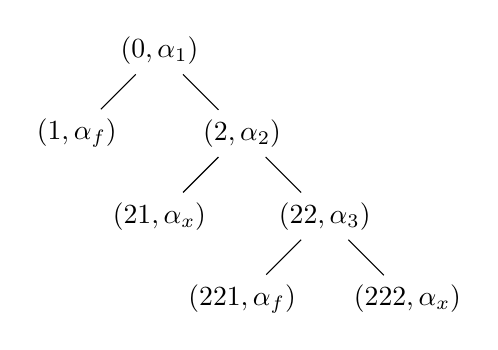
\begin{tikzpicture}[level distance=1.5cm,
  level 1/.style={sibling distance=3cm},
  level 2/.style={sibling distance=3cm}, scale=0.7]
  \node{$(0,\alpha_1)$}
  child { node {$(1, \alpha_f)$}}
  child { node {$(2, \alpha_2)$} 
     child { node {$(21, \alpha_x)$}}
         child { node {$(22, \alpha_3)$} 
           child { node {$(221,\alpha_f)$ } }
           child { node {$(222, \alpha_x)$} }
          }
      }
   ;
\end{tikzpicture} 
\end{center}

  \item Collecte des contraintes avec la fonction $T: \mathrm{terme} \mapsto \mathrm{type}$ 
    \begin{itemize}
      \item Pour une abstraction :  $e = \lambda x.e_1 $ \imp\ $T(e) = T(x) \rightarrow T(e_1) $
      \item Pour une application :  $e = e_1 e_2$ \imp\ $T(e_1) = T(e_2) \rightarrow T(e) $
      \item Pour l'application de l'addition  : $e=e_1+e_2$ \imp\ $T(e)= T(e_1) = T(e_2) = \mathtt{int} $
    \end{itemize}  

\begin{Verbatim}
utop#  t ;;
- : terme = Lam ("f", Lam ("x", App (Var "f", Var "x")))

utop# hm t ;;
- : (ltype * ltype) list =
[(Vart "alpha_1", Fleche (Vart "alpha_f", Vart "alpha_2"));
 (Vart "alpha_f", Vart "alpha_f");
 (Vart "alpha_2", Fleche (Vart "alpha_x", Vart "alpha_3"));
 (Vart "alpha_x", Vart "alpha_x");
 (Vart "alpha_f", Fleche (Vart "alpha_x", Vart "alpha_3"));
 (Vart "alpha_f", Vart "alpha_f"); (Vart "alpha_x", Vart "alpha_x")]
\end{Verbatim}
    
  \item Unification de ces constraintes afin de trouver la substitution la plus générale si l'expression est typable. 
  Dans le cas contraire, échec. Nous utilisons l'algorithme d'unification que nous détaillerons dans un chapitre suivant.

  \item Nous appliquons cette substitution à la variable de type initialement affectée au terme $t$, à l'étape 1.
\begin{Verbatim}
  - : ltype = Fleche (Fleche (Vart "alpha_x", Vart "alpha_3"),
                      Fleche (Vart "alpha_x", Vart "alpha_3"))
\end{Verbatim}
\end{enumerate}

\section{Les \textit{Pure Type Systems}}
  \subsection{Introduction}
Le $\lambda$-calcul simplement typé que nous nommons $\lambda _\rightarrow$ ne permet
de représenter des fonctions que des termes vers les termes. De manière générale, nous souhaiterions
pouvoir modéliser :
\begin{itemize}
  \item Fonction des termes vers les termes 
  \item Fonction des types vers les termes pour permettre le polymorphisme
  \item Fonction des types vers les types pour avoir des constructeurs de type 
  \item Fonction des termes vers les types pour avoir des types dépendants
\end{itemize}
Nous reprenons ici le très bon formalisme de Barendregt \cite{baren}
\begin{definition}
  La syntaxe est la suivante :
  $$ \mathcal{T} ::= V \,|\, C \,|\,\mathcal{T} \,| \,\mathcal{T} 
  \,|\, \lambda V:\mathcal{T}.\mathcal{T} \,|\, \Pi V : \mathcal{T}.\mathcal{T}
  $$
  $C$ est l'ensemble des deux constantes : $*$ et $\square$ \\
  $V$ est un ensemble fini de variables \\
  $\lambda$ est l'opération d'abstraction \\
  $\Pi$ est l'opérateur produit permettant de matérialiser le type dépendant 
\end{definition}
Il n'y a donc pas de distinction entre les termes et les types. Chaque terme est typé, chaque type est typé, avec un système pyramidal
infini.

Nous utiliserons le formalisme \textit{à la Church}.
Chaque terme est annoté de son type, contrairement au $\lambda$-calcul simplement typé 
\textit{à la Curry} que nous
avons présenté précedemment où les termes étaient libres de type et un mécanisme d'inférence de 
type permettait ensuite d'associer à chaque terme un type.

L'environnement de type $\Gamma$ est défini par :
$$ \Gamma ::= \emptyset\ |\  \Gamma, x:\mathcal{T} $$
Nous avons les règles de réduction suivantes:
$$
\begin{array}{l}
 \dfrac {}{(\lambda x:A.B)~C\to _{\beta }B[C/x]} \\[1cm]
 

\dfrac {B\to _{\beta }B'}{\lambda x:A.B\to _{\beta }\lambda x:A.B'} \\[1cm]


\dfrac {A\to _{\beta }A'}{\lambda x:A.B\to _{\beta }\lambda x:A'.B} \\[1cm]


\dfrac {B\to _{\beta }B'}{\Pi x:A.B\to _{\beta }\Pi x:A.B'} \\[1cm]


\dfrac {A\to _{\beta }A'}{\Pi x:A.B\to _{\beta }\Pi x:A'.B} \\[1cm]
  
\end{array}
$$
Nous avons les règles de typage suivantes.
\[
\begin{array}{l}

\dfrac {}{\vdash *:\square }\quad {\text{(Axiom)}}\\[1cm]

\dfrac {\Gamma \vdash A:s\quad x{\text{ does not occur in }}\Gamma }{\Gamma ,x:A\vdash x:A}\quad {\text{(Start)}}\\[1cm]

\dfrac {\Gamma \vdash A:B\quad \Gamma \vdash C:s}{\Gamma ,x:C\vdash A:B}\quad {\text{(Weakening)}}\\[1cm]

\dfrac {\Gamma \vdash C:\Pi x:A.B\quad \Gamma \vdash a:A}{\Gamma \vdash Ca:B[a/x]}\quad {\text{(Application)}}\\[1cm]

\dfrac {\Gamma \vdash A:B\quad B=_{\beta }B'\quad \Gamma \vdash B':s}{\Gamma \vdash A:B'}\quad {\text{(Conversion)}}\\[1cm]
\end{array}
\]

Soit la paire $( s 1 , s 2 ) $, nous avons les deux règles ci-dessous:
$$
\begin{array}{l}

\dfrac {\Gamma \vdash A:s_{1}\quad \Gamma ,x:A\vdash B:s_{2}}{\Gamma \vdash \Pi x:A.B:s_{2}}\quad {\text{(Product)}} \\[1cm]

\dfrac {\Gamma \vdash A:s_{1}\quad \Gamma ,x:A\vdash b:B\quad \Gamma ,x:A\vdash B:s_{2}}{\Gamma \vdash \lambda x:A.b:\Pi x:A.B}\quad {\text{(Abstraction)}}
\end{array}
$$
\vspace{0.5cm}


Le système \textit{PTS} respecte les propriétés suivantes:
\begin{enumerate}
  \item 
     La propriété de Church-Rosser :  $M\to _{\beta }N\  \text{et}\ M\to _{\beta }N'\ \text{alors il existe}\ N'' 
     \ \text{tel que}\\
      N\ \to _{\beta }^{*}N'' \text{ et } N'\to _{\beta }^{*}N''$ \\
  \item 
    La propriété de réduction : $\Gamma \vdash M:T\  \text{et}\ 
    M\to _{\beta }M' \ \text{alors}\  \Gamma \vdash M':T $ \\
    \item
    L'unicité des types : $\Gamma \vdash A:B \ \text{et}\ \Gamma \vdash A:B' \ \text{alors}\ B=_{\beta }B'$ \\
\end{enumerate}

Pour pouvoir éprouver notre système PTS, nous ajoutons les constantes suivantes à notre environnement $\Gamma$
$$\Gamma = \{ (*:\square) ;\ (\text{nat}:*) ;\ (O:nat) ;\ (\text{succ}:\Pi x:\text{nat}.\text{nat}) \} $$

Voici quelques exemples interprétés par \textsc{Ocaml} ci-dessous. Nous avons simplifié l'affichage
du type $\Pi x:A.B$ par $A\rightarrow B$ si $x$ n'est pas une variable libre de $B$.

Nous utilisons pour l'affichage \textsc{Ocaml} les caractères UTF-8 :  \verb+λ, π, →+

\begin{Verbatim}
(*  Polymorphisme   *)
let id = Lam("A", C "*", Lam("x", V "A", V "x")) ;;
let id_nat = App(id, C "nat") ;;
let zero = App(id_nat, C "O") ;;

id = λA:*.λx:A.x
id nat = λA:*.λx:A.x nat

print_terme (typage id env0) 
πA:*.A→A

print_terme (reduc id_nat) ;;
λx:nat.x

print_terme zero ;;
λA:*.λx:A.x nat O
print_terme zero ;;
print_terme (typage zero env0) ;;
nat

print_terme (fullReduc zero) ;;
O

(* Les entiers *)
let entiers = Prod ("X", C "*",  Prod ("x", V "X", Prod ("y", Prod ("z", V "X", V "X"), V "X")))
utop # print_terme entiers;;
πX:*.(X→((X→X)→X))

let zero =  Lam("X", C "*", Lam("x", V "X", Lam ("y", Prod("z", V "X", V "X"), V "x")))

let succ = Lam ("n", entiers, Lam ("X", C "*", Lam ("x", V "X", Lam ("y", Prod("z", V "X", V "X"),
               App(V "y", App (App(App(V "n", V "X"), V "x"), V "y") )))))

utop # print_terme (fullReduc trois) ;;
λX:*.λx:X.λy:(X→X).y (y (y x) ) 

(*twice*)
utop # print_terme twice ;;
λA:*.λf:(A→A).λa:A.f (f a) 

utop # print_terme (typage twice env0) ;;
πA:*.((A→A)→(A→A))

let plus2  = App(App(twice, entiers), succ) ;;
print_terme (fullReduc (App(plus2, trois))) ;
λX:*.λx:X.λy:(X→X).y (y (y (y (y x) ) ) )
\end{Verbatim}
Le type produit pourra être défini de la manière suivante :

Si $U$ et $V$ sont des types, alors 
$$U\times V = \Pi X.(U\rightarrow V \rightarrow X)\rightarrow X$$
$$ <u,v> = \lambda X:*.\lambda x:(U \rightarrow V \rightarrow X). x u v $$ 

Prenons par exemple le couple d'entiers $<100, 101>$, nous le modélisons par 
\begin{Verbatim}
let prod_100_101 = 
  Lam("X", C "nat", 
    Lam("x", Prod("z", C "nat", 
:w
     (Prod ("w", C "nat", V "X" ))),App (App (V "x", N 100), N 101))) ;;
print (typage prod_100_101 env0) ;;
πX:nat.((nat→(nat→X))→X)  
\end{Verbatim}

Les projections sont définies par 
$$\pi^1 t = t\ U (\lambda x:U.\lambda y:V. x) \text{  et  } \pi^2 t = t\ U (\lambda x:U.\lambda y:V. y)$$
\begin{Verbatim}
let proj1 = 
  Lam("t", (typage prod_uv env0), 
    App(App(V "t", V "U"), Lam ("x", V "U", Lam ("y", V "V", V "x"))))
 in print (fullReduc (App (proj1, prod_100_101)))

let proj2 = 
  Lam("t", (typage prod_uv env0),
    App(App(V "t", V "U"), Lam ("x", V "U", Lam ("y", V "V", V "y"))))
in print (fullReduc (App (proj2, prod_uv)))
\end{Verbatim}

\subsection{\textsc{MiniCoq}}
Nous  nous éloignons de la simplicité du \textit{Pure Type System} en surchargeant notre
 terme algébrique des types suivants :
\begin{itemize}
  \item Le type \verb+Nat+ avec ses constructeurs \verb+0+ et \verb+S+
  \item Le type de l'égalité \verb+Eq+ avec son unique constructeur \verb+Eq_refl+
  \item Le type \verb+And+ avec son unique constructeur \verb+Conj+ et ses fonctions
  \verb+Proj1+ et \verb+Proj2+. L'affichage du type \verb+And+ se fera avec les caractères \verb+/\+
  \item Le type \verb+Or+ avec ses constructeurs \verb+Or_introl+ et \verb+Or_intror+ et sa fonction \verb+Case+.
  L'affichage de ce type se fera avec les caractères \verb+\/+
  \item Le type \verb+False+ sans constructeur, mais avec la fonction \verb+False_ind(t1,t2)+ qui se
  réduit en \verb+t1+ si le type de \verb+t2+ est égal à \verb+False+  (\textit{ex falso quodlibet})
\end{itemize}

\vspace{0.2cm}
Démontrons le théorème simple décrit en \textsc{Coq} comme ci-dessous.


%%%%%%%%%%%%%%%%%%%%%%%%%%%%%%%%%%%%%%%%%%%%%%%%%%%%%%%%%%%%%%%%%
%% This file has been automatically generated with the command
%% coqdoc -latex imp.v 
%%%%%%%%%%%%%%%%%%%%%%%%%%%%%%%%%%%%%%%%%%%%%%%%%%%%%%%%%%%%%%%%%
\begin{coqdoccode}
\coqdocnoindent
\coqdockw{Theorem}  \coqdocvar{imp} : \coqdockw{\ensuremath{\forall}} (\coqdocvar{a} \coqdocvar{b} \coqdocvar{c} : \coqdockw{Prop}), ((\coqdocvar{a}\ensuremath{\rightarrow}\coqdocvar{b}) \ensuremath{\land} (\coqdocvar{a}\ensuremath{\rightarrow}\coqdocvar{c})) \ensuremath{\rightarrow} \coqdocvar{a}\ensuremath{\rightarrow} (\coqdocvar{b}\ensuremath{\land}\coqdocvar{c}).\coqdoceol
\coqdocnoindent
\coqdockw{Proof}.\coqdoceol
\coqdocindent{1.00em}
\coqdoctac{intros} \coqdocvar{a} \coqdocvar{b} \coqdocvar{c} \coqdocvar{H}.\coqdoceol
\coqdocindent{1.00em}
\coqdoctac{intro} \coqdocvar{Ha}.\coqdoceol
\coqdocindent{1.00em}
\coqdoctac{split}.\coqdoceol
\coqdocindent{1.00em}
\coqdoctac{destruct} \coqdocvar{H} \coqdockw{as} (\coqdocvar{H1} \& \coqdocvar{H2}).\coqdoceol
\coqdocindent{1.00em}
\coqdoctac{apply} \coqdocvar{H1}. \coqdoctac{assumption}.\coqdoceol
\coqdocindent{1.00em}
\coqdoctac{destruct} \coqdocvar{H} \coqdockw{as} (\coqdocvar{H1} \& \coqdocvar{H2}).\coqdoceol
\coqdocindent{1.00em}
\coqdoctac{apply} \coqdocvar{H2}. \coqdoctac{assumption}.\coqdoceol
\coqdocnoindent
\coqdockw{Qed}.\coqdoceol
\coqdocemptyline
\end{coqdoccode}


%%%%%%%%%%%%%%%%%%%%%%%%%%%%%%%%%%%%%%%%%%%%%%%%%%%%%%%%%%%%%%%%%%%%%%%%%%%%%%%%%%
Nous pouvons représenter la preuve du théorème avec la dérivation suivante:
\\


\begin{scriptsize}
\infer [intros\ a\ b\ c\ H]{((A\Rightarrow B)\wedge (A\Rightarrow C))\Rightarrow (A\Rightarrow (B \wedge C))}
 {\infer[intros\ Ha]{A \Rightarrow (B\wedge C)}
  {\infer[split]{B \wedge C}
   { 
      \infer[apply\ H1]{B} {\infer[destruct\ H\ as\ (H1 , H2)]{A \Rightarrow B}{[(A\Rightarrow B) \wedge (A\Rightarrow C)]} & [A] }
      & 
      \infer[apply\ H2]{C} {\infer[destruct\ H\ as\ (H1 , H2)]{A \Rightarrow C}{[(A\Rightarrow B) \wedge (A\Rightarrow C)]} & [A] }
   }
  }
 }
\end{scriptsize}
\vspace{0.2cm}

Avec notre système PTS, nous codons cela de la manière suivante:
\begin{Verbatim}
let imp = Prod("A", C "Type", Prod ("B", C "Type", Prod ("C", C "Type",
               Prod ("z", And(Prod("x", V "A", V "B"), Prod ("y", V "A", V "C")), 
                     Prod ("w", V "A", And (V "B", V "C"))))))
in print imp ;;
> πA:Type.πB:Type.π:Type.((A→B)/\(A→C)→(A→B/\C))

let preuve_imp_pts = 
 Lam("A", Type,
   Lam("B", Type,
     Lam("C", Type, 
      Lam("h", And(Prod("x", V "A", V "B"), Prod("y", V "A", V "C")), 
       Lam ("x", V "A", Conj (App(Proj1 (V "h"), V "x"), App(Proj2 (V "h"), V "x"))))))) 
in (print preuve_imp_pts; print_string "\n"; print (check preuve_imp_pts env0))  ;;

> λA:Type.λB:Type.λC:Type.λh:(A→B)/\(A→C).λx:A.conj((proj1(h) x),(proj2(h) x))
  πA:Type.πB:Type.πC:Type.((A→B)/\(A→C)→(A→B/\C))
\end{Verbatim}
Nous retrouvons en \textsc{Ocaml} la dualité entre le type produit \verb+*+ et le $\wedge$ logique,
 ainsi qu'entre la flèche fonctionnelle \verb+->+ et l'implication logique $\Rightarrow$.
\textsc{Ocaml} infère correctement le type (théorème) depuis le terme (la preuve).

\begin{Verbatim}
let preuve_imp_ocaml = function h -> (function x -> ((fst h) x, (snd h) x)) ;;
val preuve_imp_ocaml : ('a -> 'b) * ('a -> 'c) -> 'a -> 'b * 'c 
\end{Verbatim}

Voici un autre exemple très simple illustrant le type $\wedge$ et les fonctions de construction \verb+And+ et de projections \verb+Proj1/2+

%%% COQ exemple %%
\begin{coqdoccode}
\coqdocnoindent
\coqdockw{Theorem} \coqdocvar{et\_refl}: \coqdockw{\ensuremath{\forall}} (\coqdocvar{a} \coqdocvar{b}:\coqdockw{Prop}), \coqdocvar{a}\ensuremath{\land}\coqdocvar{b} \ensuremath{\rightarrow} \coqdocvar{b}\ensuremath{\land}\coqdocvar{a} .\coqdoceol
\coqdocnoindent
\coqdockw{Proof}.\coqdoceol
\coqdocindent{0.50em}
\coqdoctac{intros} \coqdocvar{a} \coqdocvar{b} \coqdocvar{H}.\coqdoceol
\coqdocindent{0.50em}
\coqdoctac{split}.\coqdoceol
\coqdocindent{0.50em}
\coqdoctac{destruct} \coqdocvar{H} \coqdockw{as} [\coqdocvar{Ha}  \coqdocvar{Hb}].\coqdoceol
\coqdocindent{0.50em}
\coqdoctac{assumption}.\coqdoceol
\coqdocindent{0.50em}
\coqdoctac{destruct} \coqdocvar{H} \coqdockw{as} [\coqdocvar{Ha} \coqdocvar{Hb}].\coqdoceol
\coqdocindent{0.50em}
\coqdoctac{assumption}.\coqdoceol
\coqdocnoindent
\coqdockw{Qed}.\coqdoceol
\coqdocemptyline
\coqdocnoindent
\coqdockw{Print} \coqdocvar{et\_refl}.\coqdoceol
\coqdocemptyline
\end{coqdoccode}

\begin{Verbatim}
let preuve_et_refl = 
  Lam("A", Type,
    Lam("B", Type, 
     Lam("h", And(V "A", V "B"), Conj(Proj2 (V "h"), Proj1 (V "h"))))) 
  in ( print preuve_et_refl ; print_string "\n"; print(check preuve_et_refl env0)) ;;
> λA:Type.λB:Type.λh:A/\B.conj(proj2(h) ,proj1(h))
  πA:Type.πB:Type.(A/\B→B/\A)
\end{Verbatim}
Ou tout simplement en \textsc{Ocaml} avec l'inférence de type:
\begin{Verbatim}
utop # let preuve_et_refl = function h -> (snd h, fst h) ;;
val preuve_et_refl : 'a * 'b -> 'b * 'a = <fun>
\end{Verbatim}

\subsection{Le $\lor$ logique}

\begin{coqdoccode}
\coqdocnoindent
\coqdockw{Theorem} \coqdocvar{or\_elim}: \coqdockw{\ensuremath{\forall}} (\coqdocvar{a} \coqdocvar{b} \coqdocvar{c}:\coqdockw{Prop}), (\coqdocvar{a}\ensuremath{\rightarrow}\coqdocvar{c})->(\coqdocvar{b}\ensuremath{\rightarrow}\coqdocvar{c})->(\coqdocvar{a}\ensuremath{\lor}\coqdocvar{b})->\coqdocvar{c}.\coqdoceol
\coqdocnoindent
\coqdockw{Proof}.\coqdoceol
\coqdocindent{1.00em}
\coqdoctac{intros} \coqdocvar{a} \coqdocvar{b} \coqdocvar{c} \coqdocvar{h1} \coqdocvar{h2} \coqdocvar{h3}.\coqdoceol
\coqdocindent{1.00em}
\coqdoctac{destruct} \coqdocvar{h3} \coqdockw{as} [\coqdocvar{ha} \ensuremath{|} \coqdocvar{hb}].\coqdoceol
\coqdocindent{1.00em}
\coqdoctac{apply} \coqdocvar{h1}. \coqdoctac{exact} \coqdocvar{ha}.\coqdoceol
\coqdocindent{1.00em}
\coqdoctac{apply} \coqdocvar{h2}. \coqdoctac{exact} \coqdocvar{hb}.\coqdoceol
\coqdocnoindent
\coqdockw{Qed}.\coqdoceol
\end{coqdoccode}
\begin{Verbatim}
(* fonction générée en COQ *)
 or_elim = 
 fun (a b c : Prop) (h1 : a -> c) (h2 : b -> c) (h3 : a \/ b) =>
 match h3 with
  | or_introl ha => h1 ha
  | or_intror hb => h2 hb
 end
     : forall a b c : Prop, (a -> c) -> (b -> c) -> a \/ b -> c  

(* fonction OCAML *)
let preuve_or_elim =
  Lam("A", Type,
    Lam("B", Type,
      Lam ("C", Type,
        Lam("h1", Prod("x", V "A", V "C"),
          Lam("h2", Prod("y", V "B", V "C"),
            Lam("h3", Or(V "A", V "B"), 
              Case(V "h3", V "h1", V "h2"))))))) 
  in (print preuve_or_elim ; print_newline() ;
      print (check preuve_or_elim env0)) ;;
> λA:Type.λB:Type.λC:Type.λh1:(A→C).λh2:(B→C).λh3:A\/B.case(h3, h1, h2)
  πA:Type.πB:Type.πC:Type.((A→C)→((B→C)→(A\/B→C)))
\end{Verbatim}

En \textsc{Ocaml}, nous introduisons le type algébrique ci-dessous pour matérialiser le \verb+or+ logique
\begin{Verbatim}
type ('a, 'b) ou = Left of 'a | Right of 'b	

let or_elim = fun h1 h2 h3 ->
 match h3 with
  | Left a -> h1 a
  | Right b -> h2 b ;;
val or_elim : ('a -> 'b) -> ('c -> 'b) -> ('a, 'c) ou -> 'b = <fun>
\end{Verbatim}

\subsection{L'égalité}
Prouvons que $\forall n \in \mathtt{Nat}, (\lambda n.2\  n) = 2$
\begin{Verbatim}
let th = Prod("n", Nat, Eq(Nat, App(cst2, V "n"), S (S O) )) 
  in print th;;
> πn:nat.eq(nat, (λn:nat.2 n), 2)

let proof = Lam("n", Nat, Eq_refl(Nat, App(cst2, V "n"))) in 
  (print proof ; print_newline() ;
   print (check proof env0) ; print_newline() ; 
   print (fullReduc (check proof env0)))  ;;
> λn:nat.eq _refl(nat, (λn:nat.2 n))
  πn:nat.eq(nat, (λn:nat.2 n), (λn:nat.2 n))
  (nat→eq(nat, 2, 2))
\end{Verbatim}
Rappelons la règle de conversion ci-dessous :
$$
\frac{\Gamma ⊢ t:A \ \ \     \Gamma ⊢ B:s \ \ \     A=_\beta B}{\Gamma ⊢ t:B}
$$
Ainsi, un terme peut avoir plusieurs types.

\noindent La preuve \verb+λn:nat.eq _refl(nat, (λn:nat.2 n))+ est preuve de :
\begin{itemize}
 \item \verb+πn:nat.eq(nat, (λn:nat.2 n), (λn:nat.2 n))+
 \item \verb+πn:nat.eq(nat, (λn:nat.2 n), 2)+
 \item \verb+(nat→eq(nat, 2, 2))+
\end{itemize}
Nous constatons que la preuve n'exhibe pas le process calculatoire de la $\beta$-réduction.
Le théorème est ici prouvé par calcul et non par raisonnement. Ces considérations philosophiques sont bien développées
par Henri Poincaré\cite{poincare}

\subsection{Le faux}

\begin{Verbatim}
let exf = Lam ("x", False, I) (* ex falso quodlibet *)
  in (print exf ; print_newline() ; print (check exf env0)) ;;
> λx:False.I
  (False→True) 
\end{Verbatim}
Voici un exemple simple manipulant la négation et la fonction d'induction du faux.  

\begin{coqdoccode}
\coqdocnoindent
\coqdockw{Theorem}  \coqdocvar{implication}: \coqdockw{\ensuremath{\forall}} (\coqdocvar{A} \coqdocvar{B}:\coqdockw{Prop}), \ensuremath{\lnot}\coqdocvar{A}\ensuremath{\lor}\coqdocvar{B} \ensuremath{\rightarrow} (\coqdocvar{A}\ensuremath{\rightarrow}\coqdocvar{B}) .\coqdoceol
\coqdocnoindent
\coqdockw{Proof}.\coqdoceol
\coqdocindent{1.00em}
\coqdoctac{intros}.\coqdoceol
\coqdocindent{1.00em}
\coqdoctac{destruct} \coqdocvar{H} \coqdockw{as} [\coqdocvar{H1}\ensuremath{|}\coqdocvar{H2}].\coqdoceol
\coqdocindent{1.00em}
\coqdocvar{contradiction}.\coqdoceol
\coqdocindent{1.00em}
\coqdoctac{assumption}.\coqdoceol
\coqdocnoindent
\coqdockw{Qed}.\coqdoceol
\coqdocemptyline
\coqdocnoindent
\coqdockw{Print} \coqdocvar{implication}.\coqdoceol
\begin{Verbatim}
implication = 
 fun (A B : Prop) (H : ~ A \/ B) (H0 : A) =>
  match H with
  | or_introl H1 => False_ind B (H1 H0)
  | or_intror H2 => H2
  end
   : forall A B : Prop, ~ A \/ B -> A -> B
\end{Verbatim}
\end{coqdoccode}


Avec notre implémentation \textsc{Ocaml}, cela donne :
\begin{Verbatim}
let preuve_impl =
  Lam("A", Type,
    Lam("B", Type,
      Lam("H", Or(App(non, V "A"), V "B"),
        Lam("H0", V "A",
          Case (V "H", 
                Lam("x", Prod("w", V "A", False), False_ind(V "B", App(V "x", V "H0"))),
                Lam ("y", V "B", V "y")))))) 
in  (print preuve_impl ; print_newline() ;
     print (fullReduc (check preuve_impl env0))) ;;
> λA:Type.λB:Type.λH:(λP:Type.~P A)\/B.λH0:A.case(H, λx:~A.false_ind(B,(x H0)), λy:B.y)
  πA:Type.πB:Type.(~A\/B→(A→B))
\end{Verbatim}

Dans un langage comme \textsc{Ocaml}, le type \verb+faux+ est un type sans constructeur.
Il est \textit{inhabité}. La preuve de la règle du modus tollens s'écrira de la manière suivante :
\begin{Verbatim}
type faux = | ;;

let modus_tollens (hfq:'q->faux) (hpq:'p->'q) (hp:'p) =
  hfq (hpq hp)
\end{Verbatim}
Voici le même théorème en \textsc{Coq} :
\begin{Verbatim}
Theorem modus_tollens: forall (p q:Prop), (q->False)-> (p->q) -> (p->False).
Proof.
	intros p q Hfq Hpq Hp.
        generalize (Hpq Hp).
        exact Hfq.
Qed.
\end{Verbatim}
Nous pouvons décrire le \textit{ex falso quodlibet} en \textsc{Ocaml} comme suit :
\begin{Verbatim}
type faux = | ;;
type vrai = I ;;

let exfalsoquodlibet = fun (f:faux) ->  I;;
\end{Verbatim}
En \textsc{Coq}, le pattern matching sur un type n'ayant aucun constructeur permet de 
définir une fonction retournant un terme de n'importe quel type.


Considérons par exemple la fonction $f$ de type $False \rightarrow 2=3$ :
\begin{Verbatim}
Definition f := fun (x:False) => 
   match x return 2=3 with end.
\end{Verbatim}
Cette fonction $f$, est à mon sens, l'expression peu élégante de la correspondance 
de Curry-Howard. Une fonction ne pouvant matcher son argument peut retourner un type non habité\dots

En \textsc{Ocaml}, je ne pense pas que la syntaxe nous permet d'écrire qu'un pattern matching
ne retourne rien, nous pouvons cependant boucler indéfiniment :
\begin{Verbatim} 
type faux = | ;;
type farfelu = | ;;
let rec f (x:faux):farfelu = f x  ;;
val f : faux -> farfelu = <fun>
\end{Verbatim}

\subsection{Le point fixe}
Nous surchargeons notre terme algébrique de l'opérateur de point fixe \verb+Y of terme+ qui
se réduit en \verb+Y t+ \imp\ \verb+t (Y t)+
\begin{Verbatim}
let multF = 
  Lam ("f", Prod("w",Nat, Nat),
   Lam ("n", Nat, Lam ("m", Nat, 
        IfThenElse(Egal(V "n",O), O, Add (V "m", App(App (V "f", Sub1 (V "n")), V "m"))))))

let mult = Y multF ;;

let facF = Lam("f", Prod ("z", Nat, Nat), 
             Lam ("n", Nat,
              IfThenElse(Egal(V "n", O), S O, (App(App(mult, V "n"), App(V "f", Sub1 (V "n")) ) )))) ;;

let fac = Y facF  ;;

print (fullReduc (App(fac, S (S (S (S (S O))))))) ;;
> 120
\end{Verbatim}

\subsection{La logique classique}
Sous l'angle de la correspondance de Curry-Howard, notre système se base sur la logique intuitionniste.
C'est-à-dire que toute proposition a une preuve constructive.
 Autrement dit, le type correspondant à la proposition est habité par un terme de notre système PTS.
Avec cette logique nous ne pouvons prouver certains théorèmes comme la loi de Peirce $((A\rightarrow B)\rightarrow A)\rightarrow A$

Pour cela nous devons ajouter l'axiome du tiers-exclus $A \vee \neg A$. 
Voici comment la loi de Pierce se déduit avec l'axiome du tiers-exclus. En \textsc{Coq}, cela donne:

\begin{coqdoccode}
\coqdocnoindent
\coqdockw{Axiom} \coqdocvar{classic}: \coqdockw{\ensuremath{\forall}} \coqdocvar{P}: \coqdockw{Prop}, \coqdocvar{P}\symbol{92}/\~{}\coqdocvar{P}.\coqdoceol
\coqdocnoindent
\coqdockw{Theorem}  \coqdocvar{Peirce}: \coqdockw{\ensuremath{\forall}} \coqdocvar{A} \coqdocvar{B}:\coqdockw{Prop}, ((\coqdocvar{A}\ensuremath{\rightarrow}\coqdocvar{B})->\coqdocvar{A})->\coqdocvar{A}.\coqdoceol
\coqdocnoindent
\coqdockw{Proof}.\coqdoceol
\coqdocindent{1.00em}
\coqdoctac{intros}.\coqdoceol
\coqdocindent{1.00em}
\coqdoctac{assert} (\coqdocvar{A}\symbol{92}/\~{}\coqdocvar{A}) \coqdoctac{by} (\coqdoctac{apply} \coqdocvar{classic} ).\coqdoceol
\coqdocindent{1.00em}
\coqdoctac{destruct} \coqdocvar{H0} \coqdockw{as} [\coqdocvar{H1} \ensuremath{|} \coqdocvar{H2}].\coqdoceol
\coqdocindent{1.00em}
\coqdoctac{exact} \coqdocvar{H1}.\coqdoceol
\coqdocindent{1.00em}
\coqdoctac{apply} \coqdocvar{H} .\coqdoceol
\coqdocindent{1.00em}
\coqdoctac{intros}.\coqdoceol
\coqdocindent{1.00em}
\coqdocvar{contradiction}.\coqdoceol
\coqdocnoindent
\coqdockw{Qed}.\coqdoceol
\coqdocemptyline
\coqdocnoindent
\coqdockw{Print} \coqdocvar{Peirce}.\coqdoceol
\end{coqdoccode}

\begin{Verbatim}
 Peirce = 
  fun (A B : Prop) (H : (A -> B) -> A) =>
  let H0 : A \/ ~ A := classic A in
  match H0 with
  | or_introl H1 => H1
  | or_intror H2 => H (fun H1 : A => False_ind B (H2 H1))
  end
    : forall A B : Prop, ((A -> B) -> A) -> A
\end{Verbatim}

Voici notre implémentation dans notre \textsc{MiniCoq}. 
Nous créons un environnement \verb+env_classic+ surchargé par le terme \verb+tiers-exclus+ de type $A \vee \neg A$.
Nous trichons un peu car le type devrait être polymorphe et donc de la forme $\forall P:\mathtt{Type}, P \vee \neg P$, mais 
je ne vois pas comment ensuite appliquer cet axiome à une variable \verb+A+. Comment \textsc{Coq} gère \verb+let H0 : A \/ ~ A := classic A+ ? 

\begin{Verbatim}
let env_classic = [("tiers-exclus",  Or(V "A", App(non, V "A")))] ;;

let proof_peirce = 
  Lam("A", Type,
    Lam("B", Type, 
      Lam ("H", Prod("x", Prod("y", V "A", V "B"), V "A"),
        Case(C "tiers-exclus",
             Lam("zz", V "A", V "zz"),
             Lam("yy", V "A", App(V "H", Lam("H1", V "A", False_ind(V "B", App(V "yy", V "H1")))))))))
  in (print proof_peirce; print_newline();
    print (check proof_peirce env_classic)) ;;
> λA:Type.λB:Type.λH:((A→B)→A).case(tiers-exclus,
                                    λzz:A.zz,
                                    λyy:A.(H λH1:A.false_ind(B,(yy H1))))
  πA:Type.πB:Type.(((A→B)→A)→A)
\end{Verbatim}
%%%%%%%%%%%%%%%%%%%%%%%%%%%%%%%%%%% %
%%%%%%%%%%%%%%%%%%%%%%%%%%%%%%%%%%%%

Ainsi, le tiers-exclus n'est pas démontrable en logique classique. Cependant, on peut
démontrer en logique intuitionniste qu'il n'est pas vrai que le tiers-exclus soit faux.
C'est-à-dire que l'on ne peut démontrer $P$, mais $\lnot\ \lnot P$

Il est surprenant de constater que "nier deux fois" est équivalent à "affirmer" en logique classique, mais est plus
faible en logique intuitionniste.

Voici la démonstration en \textsc{Coq}.

\begin{coqdoccode}
\coqdocnoindent
\coqdockw{Section} \coqdocvar{excluded\_middle}.\coqdoceol
\coqdocnoindent
\coqdockw{Variables} \coqdocvar{A} : \coqdockw{Prop}.\coqdoceol
\coqdocemptyline
\coqdocnoindent
\coqdockw{Theorem} \coqdocvar{il\_n\_est\_pas\_vrai\_que\_le\_tiers\_exclus\_est\_faux}: \ensuremath{\lnot} \ensuremath{\lnot} (\~{}\coqdocvar{A} \ensuremath{\lor} \coqdocvar{A}).\coqdoceol
\coqdocnoindent
\coqdockw{Proof}.\coqdoceol
\coqdocindent{1.00em}
\coqdoctac{unfold} \coqdocvar{not}.\coqdoceol
\coqdocindent{1.00em}
\coqdoctac{intro} \coqdocvar{H}.\coqdoceol
\coqdocindent{1.00em}
\coqdoctac{apply} \coqdocvar{H}.\coqdoceol
\coqdocindent{1.00em}
\coqdoctac{left}.\coqdoceol
\coqdocindent{1.00em}
\coqdoctac{intro} \coqdocvar{H1}.\coqdoceol
\coqdocemptyline
\coqdocindent{1.00em}
\coqdoctac{apply} \coqdocvar{H}.\coqdoceol
\coqdocindent{1.00em}
\coqdoctac{right}.\coqdoceol
\coqdocindent{1.00em}
\coqdoctac{assumption}.\coqdoceol
\coqdocnoindent
\coqdockw{Qed}.\coqdoceol
\coqdocemptyline
\coqdocnoindent
\coqdockw{End} \coqdocvar{excluded\_middle}.\coqdoceol
\end{coqdoccode}
%%%%%%%%%%%%%%%%%%%%%%%%%%%%%%%%%%% %